\chapter{A rendszer felhasználása}
\label{chap:felhasznalas}

Ez a fejezet az elkészült hangszerfelismerő rendszer gyakorlati alkalmazását mutatja be a végfelhasználó szempontjából. Részletesen ismertetem a szoftver indításának menetét, a terminál alapú interaktív felhasználói felület (CLI Dashboard) felépítését és színkódolását, valamint bemutatok több tipikus valós idejű működési forgatókönyvet (tesztesetet) szöveges konzol-mockupokon keresztül.

\section{Az alkalmazás indítása és konfigurációja}
\label{sec:inditas}

A rendszer tervezése során kiemelt szempont volt a könnyű hordozhatóság és az alacsony erőforrás-igény. Mivel a szoftver egy interaktív, valós idejű parancssori felületen fut, nincs szükség erőforrás-igényes grafikus ablakkezelő rendszerek betöltésére, így az alkalmazás akár szervereken vagy korlátozott teljesítményű beágyazott eszközökön is futtatható.

Az indítás előfeltételei az alábbiak:
\begin{enumerate}
    \item A virtuális környezet aktiválása a projekt gyökérkönyvtárában:
\begin{lstlisting}
source venv/bin/activate
\end{lstlisting}
    \item A külső mikrofon vagy a beépített hangbemeneti eszköz csatlakoztatása és alapértelmezetté tétele a rendszerbeállításokban.
\end{enumerate}

Az indítás a következő parancs futtatásával történik:
\begin{lstlisting}
python scripts/05a_realtime_recognition.py
\end{lstlisting}

Az alkalmazás indításakor a konzolon megjelennek a konfigurációs paraméterek, a betanított Keras modell betöltésének állapota, valamint az élő jelfeldolgozási folyamat megkezdését jelző üzenet (lásd a \ref{fig:realtime_setup}.~ábrát):

\begin{figure}[H]
    \centering
    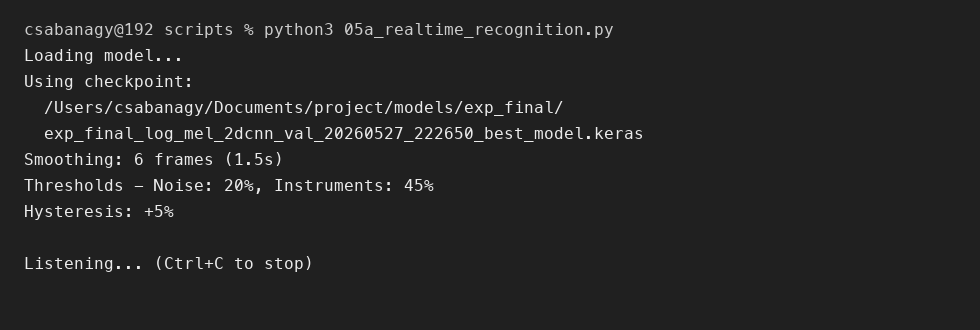
\includegraphics[width=0.75\textwidth]{fig_realtime_setup.png}
    \caption{Az alkalmazás indításakor megjelenő konfigurációs és betöltési paraméterek}
    \label{fig:realtime_setup}
\end{figure}

\section{A parancssori felhasználói felület felépítése}
\label{sec:cli_dashboard}

A valós idejű visszajelzést egy dinamikusan frissülő terminálsor (CLI Dashboard) biztosítja. A hagyományos, soronként görgető konzolos kiírás helyett a program a kocsivissza (\texttt{\textbackslash r}) karaktert használja, így a terminál egyetlen sorát írja felül folyamatosan a legfrissebb információkkal. Ez reszponzív, villódzásmentes felhasználói élményt nyújt.

A kijelző sor három fő vizuális komponensből áll:
\begin{enumerate}
    \item \textbf{Dinamikus konfidencia-sáv:} Egy 20 karakter hosszúságú grafikus sáv, amely a felismert hangszer valószínűségét ábrázolja vizuálisan. 
    \item \textbf{Aktív osztály és konfidencia érték:} A felismert hangszer megnevezése és a kiszámított valószínűségi százalékos érték (tizedes pontossággal). A kijelzőn látható aktív kategória csak akkor vált át egy új hangszerre vagy csendre, ha annak simított valószínűsége a háttérben meghaladja a beépített biztonsági küszöbértéket (hangszerek esetén $45\%$, zaj/csend esetén $20\%$). Ezzel biztosítja a program a stabil vizuális visszajelzést.
    \item \textbf{Másodlagos osztályok valószínűségei:} A többi hangszerosztály rövidített jelölése (G: Gitár, P: Zongora, V: Vokál, S: Vonós, R: Nádfúvós, B: Rézfúvós, N: Zaj/Csend) és azok pillanatnyi valószínűségi értékei, amelyek segítenek a felhasználónak átlátni a modell bizonytalansági tényezőit és az átfedéseket.
\end{enumerate}

\subsection{ANSI színkódolás és jelölések}

A felület a terminál ANSI escape szekvenciáit kihasználva színesben jeleníti meg a felismert hangszereket. Minden hangszerosztály egyedi, kontrasztos színt kapott, így a felhasználó akár távolabbról, a szöveg elolvasása nélkül is azonnal látja az aktív hangszert. A színkódokat, jelöléseket és az osztályok leírását a \ref{tab:ansi_colors}.~táblázat foglalja össze:

\begin{table}[H]
\centering
\caption{A parancssori felületen alkalmazott ANSI színkódok és rövidítések kategóriánként}
\label{tab:ansi_colors}
\begin{tabular}{llcl}
\toprule
\textbf{Kategória} & \textbf{Terminál színe} & \textbf{Rövidítés} & \textbf{Leírás} \\
\midrule
\texttt{guitar} & Sárga & G & Pengetős hangszerek (pl. akusztikus gitár) \\
\texttt{piano} & Inverz Fekete/Fehér & P & Billentyűs hangszerek (zongora) \\
\texttt{vocal} & Ciánkék & V & Emberi énekhang (vokál) \\
\texttt{string} & Sötétvörös & S & Vonós hangszerek \\
\texttt{reed} & Narancssárga & R & Nádas fúvós hangszerek (szaxofon) \\
\texttt{brass} & Világosbarna & B & Rézfúvós hangszerek \\
\texttt{noise} & Szürke & N & Környezeti zaj / csend \\
\bottomrule
\end{tabular}
\end{table}

\section{Működési forgatókönyvek és tesztesetek}
\label{sec:forgatokonyvek}

Az alábbiakban bemutatom, hogyan reagál a konzolos interfész a különböző akusztikai bemenetekre valós időben.

\subsection{1. teszteset: Csendes szobai környezet (alapállapot)}
Amikor a szobában nincs aktív hangszeres játék, csak a számítógép ventilátora vagy távoli környezeti zörejek hallatszanak, az RMS zajkapu átengedi a jelet (vagy a modell zajként azonosítja), így a szürke színű \texttt{noise} osztály válik aktívvá kiugróan magas konfidenciával. A terminál kijelzése ekkor a \ref{fig:realtime_noise}.~ábrán látható:

\begin{figure}[H]
    \centering
    
\includegraphics[width=0.6\textwidth]{fig_realtime_noise.png}
    \caption{A rendszer kimenete csendes szobai környezet (zaj) esetén}
    \label{fig:realtime_noise}
\end{figure}

\subsection{2. teszteset: Akusztikus gitárjáték (monofón dallam)}
Amikor a felhasználó megszólaltat egy akusztikus gitárt a mikrofon közelében, a modell az első ablak után azonnal reagál. A simító ablaknak ($2,0$ másodperc) és a hiszterézisnek köszönhetően a kijelzés stabilan átvált sárga színű \texttt{guitar} feliratra, miközben a többi hangszer valószínűsége minimálisra csökken (lásd a \ref{fig:realtime_guitar}.~ábrát):

\begin{figure}[H]
    \centering
    
\includegraphics[width=0.6\textwidth]{fig_realtime_guitar.png}
    \caption{A rendszer kimenete akusztikus gitárjáték érzékelésekor}
    \label{fig:realtime_guitar}
\end{figure}

\subsection{3. teszteset: Emberi énekhang (vokál)}
Amikor a felhasználó énekelni vagy beszélni kezd a mikrofonba, a kijelző azonnal ciánkékre vált, és a \texttt{vocal} osztály jelenik meg. Mivel az ének felhangjai nagyon tiszták és erősek, a konfidencia érték gyorsan emelkedik (lásd a \ref{fig:realtime_vocal}.~ábrát):

\begin{figure}[H]
    \centering
    
\includegraphics[width=0.6\textwidth]{fig_realtime_vocal.png}
    \caption{A rendszer kimenete emberi énekhang (vokál) érzékelésekor}
    \label{fig:realtime_vocal}
\end{figure}

\subsection{4. teszteset: Szaxofon játék (átmeneti bizonytalanság)}
Amikor a felhasználó szaxofonon játszik, a modell kezdetben a rézfúvós és nádfúvós osztályok között oszcillálhat az akusztikai hasonlóságok miatt. A hiszterézis bónusz és a konfidencia-küszöb azonban stabilizálja az eredményt, így a kijelző fixen narancssárga \texttt{reed} színben marad (lásd a \ref{fig:realtime_reed}.~ábrát):

\begin{figure}[H]
    \centering
    
\includegraphics[width=0.6\textwidth]{fig_realtime_reed.png}
    \caption{A rendszer kimenete szaxofon játék (reed) érzékelésekor}
    \label{fig:realtime_reed}
\end{figure}

\subsection{Az alkalmazás leállítása}
A felhasználó bármikor megszakíthatja az élő elemzést a terminálban kiadott \texttt{Ctrl+C} billentyűkombinációval. Ekkor a parancssori visszahívási szálak lezárulnak, a mikrofonbemenet felszabadul, és a program tiszta állapotban kilép a terminálba, egy rövid \texttt{Stopped.} üzenet kíséretében.
